% Created by tikzDevice version 0.12.6 on 2026-08-08 12:11:47
% !TEX encoding = UTF-8 Unicode
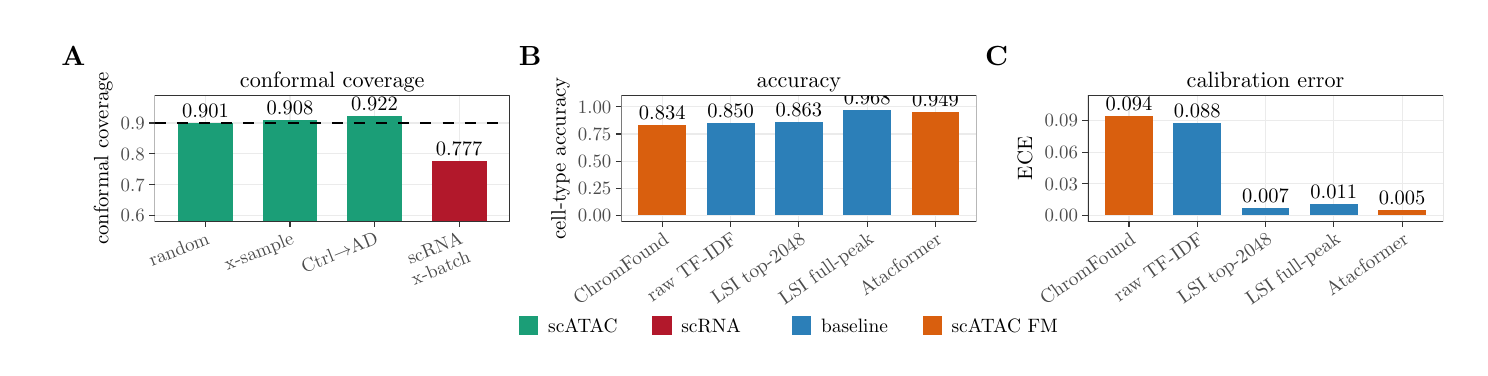
\begin{tikzpicture}[x=1pt,y=1pt]
\definecolor{fillColor}{RGB}{255,255,255}
\path[use as bounding box,fill=fillColor,fill opacity=0.00] (0,0) rectangle (517.45,115.63);
\begin{scope}
\path[clip] (  0.00,  0.00) rectangle (517.45,115.63);
\definecolor{drawColor}{RGB}{255,255,255}
\definecolor{fillColor}{RGB}{255,255,255}

\path[draw=drawColor,line width= 0.4pt,line join=round,line cap=round,fill=fillColor] (  0.00,  0.00) rectangle (517.45,115.63);
\end{scope}
\begin{scope}
\path[clip] ( 12.00,  2.00) rectangle (177.22,107.63);
\definecolor{drawColor}{RGB}{255,255,255}
\definecolor{fillColor}{RGB}{255,255,255}

\path[draw=drawColor,line width= 0.4pt,line join=round,line cap=round,fill=fillColor] ( 12.00,  2.00) rectangle (177.22,107.63);
\end{scope}
\begin{scope}
\path[clip] (177.22,  2.00) rectangle (345.84,107.63);
\definecolor{drawColor}{RGB}{255,255,255}
\definecolor{fillColor}{RGB}{255,255,255}

\path[draw=drawColor,line width= 0.4pt,line join=round,line cap=round,fill=fillColor] (177.22,  2.00) rectangle (345.84,107.63);
\end{scope}
\begin{scope}
\path[clip] (345.84,  2.00) rectangle (514.45,107.63);
\definecolor{drawColor}{RGB}{255,255,255}
\definecolor{fillColor}{RGB}{255,255,255}

\path[draw=drawColor,line width= 0.4pt,line join=round,line cap=round,fill=fillColor] (345.84,  2.00) rectangle (514.45,107.63);
\end{scope}
\begin{scope}
\path[clip] ( 45.91, 45.70) rectangle (174.22, 91.07);
\definecolor{fillColor}{RGB}{255,255,255}

\path[fill=fillColor] ( 45.91, 45.70) rectangle (174.22, 91.07);
\definecolor{drawColor}{gray}{0.92}

\path[draw=drawColor,line width= 0.4pt,line join=round] ( 45.91, 47.76) --
	(174.22, 47.76);

\path[draw=drawColor,line width= 0.4pt,line join=round] ( 45.91, 58.91) --
	(174.22, 58.91);

\path[draw=drawColor,line width= 0.4pt,line join=round] ( 45.91, 70.06) --
	(174.22, 70.06);

\path[draw=drawColor,line width= 0.4pt,line join=round] ( 45.91, 81.20) --
	(174.22, 81.20);

\path[draw=drawColor,line width= 0.4pt,line join=round] ( 64.24, 45.70) --
	( 64.24, 91.07);

\path[draw=drawColor,line width= 0.4pt,line join=round] ( 94.79, 45.70) --
	( 94.79, 91.07);

\path[draw=drawColor,line width= 0.4pt,line join=round] (125.34, 45.70) --
	(125.34, 91.07);

\path[draw=drawColor,line width= 0.4pt,line join=round] (155.89, 45.70) --
	(155.89, 91.07);
\definecolor{fillColor}{RGB}{27,158,119}

\path[fill=fillColor] ( 54.31,-19.12) rectangle ( 74.17, 81.30);

\path[fill=fillColor] ( 84.86,-19.12) rectangle (104.72, 82.11);

\path[fill=fillColor] (115.41,-19.12) rectangle (135.27, 83.67);
\definecolor{fillColor}{RGB}{178,24,43}

\path[fill=fillColor] (145.96,-19.12) rectangle (165.82, 67.49);
\definecolor{drawColor}{RGB}{0,0,0}

\path[draw=drawColor,line width= 0.4pt,dash pattern=on 4pt off 4pt ,line join=round] ( 45.91, 81.20) -- (174.22, 81.20);

\node[text=drawColor,anchor=base,inner sep=0pt, outer sep=0pt, scale=  0.74] at ( 64.24, 83.34) {0.901};

\node[text=drawColor,anchor=base,inner sep=0pt, outer sep=0pt, scale=  0.74] at ( 94.79, 84.14) {0.908};

\node[text=drawColor,anchor=base,inner sep=0pt, outer sep=0pt, scale=  0.74] at (125.34, 85.70) {0.922};

\node[text=drawColor,anchor=base,inner sep=0pt, outer sep=0pt, scale=  0.74] at (155.89, 69.53) {0.777};
\definecolor{drawColor}{gray}{0.20}

\path[draw=drawColor,line width= 0.4pt,line join=round,line cap=round] ( 45.91, 45.70) rectangle (174.22, 91.07);
\end{scope}
\begin{scope}
\path[clip] (  0.00,  0.00) rectangle (517.45,115.63);
\definecolor{drawColor}{gray}{0.30}

\node[text=drawColor,anchor=base east,inner sep=0pt, outer sep=0pt, scale=  0.68] at ( 42.31, 45.42) {0.6};

\node[text=drawColor,anchor=base east,inner sep=0pt, outer sep=0pt, scale=  0.68] at ( 42.31, 56.57) {0.7};

\node[text=drawColor,anchor=base east,inner sep=0pt, outer sep=0pt, scale=  0.68] at ( 42.31, 67.71) {0.8};

\node[text=drawColor,anchor=base east,inner sep=0pt, outer sep=0pt, scale=  0.68] at ( 42.31, 78.86) {0.9};
\end{scope}
\begin{scope}
\path[clip] (  0.00,  0.00) rectangle (517.45,115.63);
\definecolor{drawColor}{gray}{0.20}

\path[draw=drawColor,line width= 0.4pt,line join=round] ( 43.91, 47.76) --
	( 45.91, 47.76);

\path[draw=drawColor,line width= 0.4pt,line join=round] ( 43.91, 58.91) --
	( 45.91, 58.91);

\path[draw=drawColor,line width= 0.4pt,line join=round] ( 43.91, 70.06) --
	( 45.91, 70.06);

\path[draw=drawColor,line width= 0.4pt,line join=round] ( 43.91, 81.20) --
	( 45.91, 81.20);
\end{scope}
\begin{scope}
\path[clip] (  0.00,  0.00) rectangle (517.45,115.63);
\definecolor{drawColor}{gray}{0.20}

\path[draw=drawColor,line width= 0.4pt,line join=round] ( 64.24, 43.70) --
	( 64.24, 45.70);

\path[draw=drawColor,line width= 0.4pt,line join=round] ( 94.79, 43.70) --
	( 94.79, 45.70);

\path[draw=drawColor,line width= 0.4pt,line join=round] (125.34, 43.70) --
	(125.34, 45.70);

\path[draw=drawColor,line width= 0.4pt,line join=round] (155.89, 43.70) --
	(155.89, 45.70);
\end{scope}
\begin{scope}
\path[clip] (  0.00,  0.00) rectangle (517.45,115.63);
\definecolor{drawColor}{gray}{0.30}

\node[text=drawColor,rotate= 22.00,anchor=base east,inner sep=0pt, outer sep=0pt, scale=  0.68] at ( 65.99, 37.76) {random};

\node[text=drawColor,rotate= 22.00,anchor=base east,inner sep=0pt, outer sep=0pt, scale=  0.68] at ( 96.54, 37.76) {x-sample};

\node[text=drawColor,rotate= 22.00,anchor=base east,inner sep=0pt, outer sep=0pt, scale=  0.68] at (127.09, 37.76) {Ctrl$\to$AD};

\node[text=drawColor,rotate= 22.00,anchor=base east,inner sep=0pt, outer sep=0pt, scale=  0.68] at (157.64, 37.76) {scRNA};

\node[text=drawColor,rotate= 22.00,anchor=base east,inner sep=0pt, outer sep=0pt, scale=  0.68] at (160.39, 30.95) {x-batch};
\end{scope}
\begin{scope}
\path[clip] (  0.00,  0.00) rectangle (517.45,115.63);
\definecolor{drawColor}{RGB}{0,0,0}

\node[text=drawColor,rotate= 90.00,anchor=base,inner sep=0pt, outer sep=0pt, scale=  0.75] at ( 29.17, 68.38) {conformal coverage};
\end{scope}
\begin{scope}
\path[clip] (  0.00,  0.00) rectangle (517.45,115.63);
\definecolor{drawColor}{RGB}{0,0,0}

\node[text=drawColor,anchor=base,inner sep=0pt, outer sep=0pt, scale=  0.80] at (110.06, 94.12) {conformal coverage};
\end{scope}
\begin{scope}
\path[clip] (  0.00,  0.00) rectangle (517.45,115.63);
\definecolor{drawColor}{RGB}{0,0,0}

\node[text=drawColor,anchor=base,inner sep=0pt, outer sep=0pt, scale=  1.00] at ( 16.49,101.92) {\bfseries A};
\end{scope}
\begin{scope}
\path[clip] (214.53, 45.70) rectangle (342.84, 91.07);
\definecolor{fillColor}{RGB}{255,255,255}

\path[fill=fillColor] (214.53, 45.70) rectangle (342.84, 91.07);
\definecolor{drawColor}{gray}{0.92}

\path[draw=drawColor,line width= 0.4pt,line join=round] (214.53, 47.76) --
	(342.84, 47.76);

\path[draw=drawColor,line width= 0.4pt,line join=round] (214.53, 57.58) --
	(342.84, 57.58);

\path[draw=drawColor,line width= 0.4pt,line join=round] (214.53, 67.40) --
	(342.84, 67.40);

\path[draw=drawColor,line width= 0.4pt,line join=round] (214.53, 77.22) --
	(342.84, 77.22);

\path[draw=drawColor,line width= 0.4pt,line join=round] (214.53, 87.04) --
	(342.84, 87.04);

\path[draw=drawColor,line width= 0.4pt,line join=round] (229.33, 45.70) --
	(229.33, 91.07);

\path[draw=drawColor,line width= 0.4pt,line join=round] (254.01, 45.70) --
	(254.01, 91.07);

\path[draw=drawColor,line width= 0.4pt,line join=round] (278.68, 45.70) --
	(278.68, 91.07);

\path[draw=drawColor,line width= 0.4pt,line join=round] (303.36, 45.70) --
	(303.36, 91.07);

\path[draw=drawColor,line width= 0.4pt,line join=round] (328.03, 45.70) --
	(328.03, 91.07);
\definecolor{fillColor}{RGB}{217,95,14}

\path[fill=fillColor] (220.70, 47.76) rectangle (237.97, 80.52);
\definecolor{fillColor}{RGB}{44,127,184}

\path[fill=fillColor] (245.37, 47.76) rectangle (262.64, 81.16);

\path[fill=fillColor] (270.05, 47.76) rectangle (287.32, 81.66);

\path[fill=fillColor] (294.72, 47.76) rectangle (311.99, 85.79);
\definecolor{fillColor}{RGB}{217,95,14}

\path[fill=fillColor] (319.39, 47.76) rectangle (336.67, 85.02);
\definecolor{drawColor}{RGB}{0,0,0}

\node[text=drawColor,anchor=base,inner sep=0pt, outer sep=0pt, scale=  0.74] at (229.33, 82.55) {0.834};

\node[text=drawColor,anchor=base,inner sep=0pt, outer sep=0pt, scale=  0.74] at (254.01, 83.20) {0.850};

\node[text=drawColor,anchor=base,inner sep=0pt, outer sep=0pt, scale=  0.74] at (278.68, 83.69) {0.863};

\node[text=drawColor,anchor=base,inner sep=0pt, outer sep=0pt, scale=  0.74] at (303.36, 87.83) {0.968};

\node[text=drawColor,anchor=base,inner sep=0pt, outer sep=0pt, scale=  0.74] at (328.03, 87.06) {0.949};
\definecolor{drawColor}{gray}{0.20}

\path[draw=drawColor,line width= 0.4pt,line join=round,line cap=round] (214.53, 45.70) rectangle (342.84, 91.07);
\end{scope}
\begin{scope}
\path[clip] (  0.00,  0.00) rectangle (517.45,115.63);
\definecolor{drawColor}{gray}{0.30}

\node[text=drawColor,anchor=base east,inner sep=0pt, outer sep=0pt, scale=  0.68] at (210.93, 45.42) {0.00};

\node[text=drawColor,anchor=base east,inner sep=0pt, outer sep=0pt, scale=  0.68] at (210.93, 55.24) {0.25};

\node[text=drawColor,anchor=base east,inner sep=0pt, outer sep=0pt, scale=  0.68] at (210.93, 65.06) {0.50};

\node[text=drawColor,anchor=base east,inner sep=0pt, outer sep=0pt, scale=  0.68] at (210.93, 74.88) {0.75};

\node[text=drawColor,anchor=base east,inner sep=0pt, outer sep=0pt, scale=  0.68] at (210.93, 84.70) {1.00};
\end{scope}
\begin{scope}
\path[clip] (  0.00,  0.00) rectangle (517.45,115.63);
\definecolor{drawColor}{gray}{0.20}

\path[draw=drawColor,line width= 0.4pt,line join=round] (212.53, 47.76) --
	(214.53, 47.76);

\path[draw=drawColor,line width= 0.4pt,line join=round] (212.53, 57.58) --
	(214.53, 57.58);

\path[draw=drawColor,line width= 0.4pt,line join=round] (212.53, 67.40) --
	(214.53, 67.40);

\path[draw=drawColor,line width= 0.4pt,line join=round] (212.53, 77.22) --
	(214.53, 77.22);

\path[draw=drawColor,line width= 0.4pt,line join=round] (212.53, 87.04) --
	(214.53, 87.04);
\end{scope}
\begin{scope}
\path[clip] (  0.00,  0.00) rectangle (517.45,115.63);
\definecolor{drawColor}{gray}{0.20}

\path[draw=drawColor,line width= 0.4pt,line join=round] (229.33, 43.70) --
	(229.33, 45.70);

\path[draw=drawColor,line width= 0.4pt,line join=round] (254.01, 43.70) --
	(254.01, 45.70);

\path[draw=drawColor,line width= 0.4pt,line join=round] (278.68, 43.70) --
	(278.68, 45.70);

\path[draw=drawColor,line width= 0.4pt,line join=round] (303.36, 43.70) --
	(303.36, 45.70);

\path[draw=drawColor,line width= 0.4pt,line join=round] (328.03, 43.70) --
	(328.03, 45.70);
\end{scope}
\begin{scope}
\path[clip] (  0.00,  0.00) rectangle (517.45,115.63);
\definecolor{drawColor}{gray}{0.30}

\node[text=drawColor,rotate= 35.00,anchor=base east,inner sep=0pt, outer sep=0pt, scale=  0.70] at (232.10, 38.15) {ChromFound};

\node[text=drawColor,rotate= 35.00,anchor=base east,inner sep=0pt, outer sep=0pt, scale=  0.70] at (256.77, 38.15) {raw TF-IDF};

\node[text=drawColor,rotate= 35.00,anchor=base east,inner sep=0pt, outer sep=0pt, scale=  0.70] at (281.45, 38.15) {LSI top-2048};

\node[text=drawColor,rotate= 35.00,anchor=base east,inner sep=0pt, outer sep=0pt, scale=  0.70] at (306.12, 38.15) {LSI full-peak};

\node[text=drawColor,rotate= 35.00,anchor=base east,inner sep=0pt, outer sep=0pt, scale=  0.70] at (330.80, 38.15) {Atacformer};
\end{scope}
\begin{scope}
\path[clip] (  0.00,  0.00) rectangle (517.45,115.63);
\definecolor{drawColor}{RGB}{0,0,0}

\node[text=drawColor,rotate= 90.00,anchor=base,inner sep=0pt, outer sep=0pt, scale=  0.75] at (194.38, 68.38) {cell-type accuracy};
\end{scope}
\begin{scope}
\path[clip] (  0.00,  0.00) rectangle (517.45,115.63);
\definecolor{drawColor}{RGB}{0,0,0}

\node[text=drawColor,anchor=base,inner sep=0pt, outer sep=0pt, scale=  0.80] at (278.68, 94.12) {accuracy};
\end{scope}
\begin{scope}
\path[clip] (  0.00,  0.00) rectangle (517.45,115.63);
\definecolor{drawColor}{RGB}{0,0,0}

\node[text=drawColor,anchor=base,inner sep=0pt, outer sep=0pt, scale=  1.00] at (181.54,101.92) {\bfseries B};
\end{scope}
\begin{scope}
\path[clip] (383.14, 45.70) rectangle (511.45, 91.07);
\definecolor{fillColor}{RGB}{255,255,255}

\path[fill=fillColor] (383.14, 45.70) rectangle (511.45, 91.07);
\definecolor{drawColor}{gray}{0.92}

\path[draw=drawColor,line width= 0.4pt,line join=round] (383.14, 47.76) --
	(511.45, 47.76);

\path[draw=drawColor,line width= 0.4pt,line join=round] (383.14, 59.22) --
	(511.45, 59.22);

\path[draw=drawColor,line width= 0.4pt,line join=round] (383.14, 70.67) --
	(511.45, 70.67);

\path[draw=drawColor,line width= 0.4pt,line join=round] (383.14, 82.13) --
	(511.45, 82.13);

\path[draw=drawColor,line width= 0.4pt,line join=round] (397.95, 45.70) --
	(397.95, 91.07);

\path[draw=drawColor,line width= 0.4pt,line join=round] (422.62, 45.70) --
	(422.62, 91.07);

\path[draw=drawColor,line width= 0.4pt,line join=round] (447.30, 45.70) --
	(447.30, 91.07);

\path[draw=drawColor,line width= 0.4pt,line join=round] (471.97, 45.70) --
	(471.97, 91.07);

\path[draw=drawColor,line width= 0.4pt,line join=round] (496.65, 45.70) --
	(496.65, 91.07);
\definecolor{fillColor}{RGB}{217,95,14}

\path[fill=fillColor] (389.31, 47.76) rectangle (406.59, 83.62);
\definecolor{fillColor}{RGB}{44,127,184}

\path[fill=fillColor] (413.99, 47.76) rectangle (431.26, 81.29);

\path[fill=fillColor] (438.66, 47.76) rectangle (455.94, 50.47);

\path[fill=fillColor] (463.34, 47.76) rectangle (480.61, 51.89);
\definecolor{fillColor}{RGB}{217,95,14}

\path[fill=fillColor] (488.01, 47.76) rectangle (505.28, 49.79);
\definecolor{drawColor}{RGB}{0,0,0}

\node[text=drawColor,anchor=base,inner sep=0pt, outer sep=0pt, scale=  0.74] at (397.95, 85.66) {0.094};

\node[text=drawColor,anchor=base,inner sep=0pt, outer sep=0pt, scale=  0.74] at (422.62, 83.33) {0.088};

\node[text=drawColor,anchor=base,inner sep=0pt, outer sep=0pt, scale=  0.74] at (447.30, 52.51) {0.007};

\node[text=drawColor,anchor=base,inner sep=0pt, outer sep=0pt, scale=  0.74] at (471.97, 53.92) {0.011};

\node[text=drawColor,anchor=base,inner sep=0pt, outer sep=0pt, scale=  0.74] at (496.65, 51.82) {0.005};
\definecolor{drawColor}{gray}{0.20}

\path[draw=drawColor,line width= 0.4pt,line join=round,line cap=round] (383.14, 45.70) rectangle (511.45, 91.07);
\end{scope}
\begin{scope}
\path[clip] (  0.00,  0.00) rectangle (517.45,115.63);
\definecolor{drawColor}{gray}{0.30}

\node[text=drawColor,anchor=base east,inner sep=0pt, outer sep=0pt, scale=  0.68] at (379.54, 45.42) {0.00};

\node[text=drawColor,anchor=base east,inner sep=0pt, outer sep=0pt, scale=  0.68] at (379.54, 56.88) {0.03};

\node[text=drawColor,anchor=base east,inner sep=0pt, outer sep=0pt, scale=  0.68] at (379.54, 68.33) {0.06};

\node[text=drawColor,anchor=base east,inner sep=0pt, outer sep=0pt, scale=  0.68] at (379.54, 79.79) {0.09};
\end{scope}
\begin{scope}
\path[clip] (  0.00,  0.00) rectangle (517.45,115.63);
\definecolor{drawColor}{gray}{0.20}

\path[draw=drawColor,line width= 0.4pt,line join=round] (381.14, 47.76) --
	(383.14, 47.76);

\path[draw=drawColor,line width= 0.4pt,line join=round] (381.14, 59.22) --
	(383.14, 59.22);

\path[draw=drawColor,line width= 0.4pt,line join=round] (381.14, 70.67) --
	(383.14, 70.67);

\path[draw=drawColor,line width= 0.4pt,line join=round] (381.14, 82.13) --
	(383.14, 82.13);
\end{scope}
\begin{scope}
\path[clip] (  0.00,  0.00) rectangle (517.45,115.63);
\definecolor{drawColor}{gray}{0.20}

\path[draw=drawColor,line width= 0.4pt,line join=round] (397.95, 43.70) --
	(397.95, 45.70);

\path[draw=drawColor,line width= 0.4pt,line join=round] (422.62, 43.70) --
	(422.62, 45.70);

\path[draw=drawColor,line width= 0.4pt,line join=round] (447.30, 43.70) --
	(447.30, 45.70);

\path[draw=drawColor,line width= 0.4pt,line join=round] (471.97, 43.70) --
	(471.97, 45.70);

\path[draw=drawColor,line width= 0.4pt,line join=round] (496.65, 43.70) --
	(496.65, 45.70);
\end{scope}
\begin{scope}
\path[clip] (  0.00,  0.00) rectangle (517.45,115.63);
\definecolor{drawColor}{gray}{0.30}

\node[text=drawColor,rotate= 35.00,anchor=base east,inner sep=0pt, outer sep=0pt, scale=  0.70] at (400.71, 38.15) {ChromFound};

\node[text=drawColor,rotate= 35.00,anchor=base east,inner sep=0pt, outer sep=0pt, scale=  0.70] at (425.39, 38.15) {raw TF-IDF};

\node[text=drawColor,rotate= 35.00,anchor=base east,inner sep=0pt, outer sep=0pt, scale=  0.70] at (450.06, 38.15) {LSI top-2048};

\node[text=drawColor,rotate= 35.00,anchor=base east,inner sep=0pt, outer sep=0pt, scale=  0.70] at (474.74, 38.15) {LSI full-peak};

\node[text=drawColor,rotate= 35.00,anchor=base east,inner sep=0pt, outer sep=0pt, scale=  0.70] at (499.41, 38.15) {Atacformer};
\end{scope}
\begin{scope}
\path[clip] (  0.00,  0.00) rectangle (517.45,115.63);
\definecolor{drawColor}{RGB}{0,0,0}

\node[text=drawColor,rotate= 90.00,anchor=base,inner sep=0pt, outer sep=0pt, scale=  0.75] at (363.00, 68.38) {ECE};
\end{scope}
\begin{scope}
\path[clip] (  0.00,  0.00) rectangle (517.45,115.63);
\definecolor{drawColor}{RGB}{0,0,0}

\node[text=drawColor,anchor=base,inner sep=0pt, outer sep=0pt, scale=  0.80] at (447.30, 94.12) {calibration error};
\end{scope}
\begin{scope}
\path[clip] (  0.00,  0.00) rectangle (517.45,115.63);
\definecolor{drawColor}{RGB}{0,0,0}

\node[text=drawColor,anchor=base,inner sep=0pt, outer sep=0pt, scale=  1.00] at (350.15,101.92) {\bfseries C};
\end{scope}
\begin{scope}
\path[clip] (  0.00,  0.00) rectangle (517.45,115.63);
\definecolor{fillColor}{RGB}{255,255,255}

\path[fill=fillColor] (176.08,  4.00) rectangle (266.71, 12.00);
\end{scope}
\begin{scope}
\path[clip] (  0.00,  0.00) rectangle (517.45,115.63);
\definecolor{fillColor}{RGB}{255,255,255}

\path[fill=fillColor] (177.08,  4.00) rectangle (185.08, 12.00);
\definecolor{fillColor}{RGB}{27,158,119}

\path[fill=fillColor] (177.59,  4.52) rectangle (184.56, 11.48);
\end{scope}
\begin{scope}
\path[clip] (  0.00,  0.00) rectangle (517.45,115.63);
\definecolor{fillColor}{RGB}{255,255,255}

\path[fill=fillColor] (225.19,  4.00) rectangle (233.19, 12.00);
\definecolor{fillColor}{RGB}{178,24,43}

\path[fill=fillColor] (225.71,  4.52) rectangle (232.67, 11.48);
\end{scope}
\begin{scope}
\path[clip] (  0.00,  0.00) rectangle (517.45,115.63);
\definecolor{drawColor}{RGB}{0,0,0}

\node[text=drawColor,anchor=base west,inner sep=0pt, outer sep=0pt, scale=  0.70] at (188.08,  5.59) {scATAC};
\end{scope}
\begin{scope}
\path[clip] (  0.00,  0.00) rectangle (517.45,115.63);
\definecolor{drawColor}{RGB}{0,0,0}

\node[text=drawColor,anchor=base west,inner sep=0pt, outer sep=0pt, scale=  0.70] at (236.19,  5.59) {scRNA};
\end{scope}
\begin{scope}
\path[clip] (  0.00,  0.00) rectangle (517.45,115.63);
\definecolor{fillColor}{RGB}{255,255,255}

\path[fill=fillColor] (274.71,  4.00) rectangle (381.29, 12.00);
\end{scope}
\begin{scope}
\path[clip] (  0.00,  0.00) rectangle (517.45,115.63);
\definecolor{fillColor}{RGB}{255,255,255}

\path[fill=fillColor] (275.71,  4.00) rectangle (283.71, 12.00);
\definecolor{fillColor}{RGB}{44,127,184}

\path[fill=fillColor] (276.23,  4.52) rectangle (283.19, 11.48);
\end{scope}
\begin{scope}
\path[clip] (  0.00,  0.00) rectangle (517.45,115.63);
\definecolor{fillColor}{RGB}{255,255,255}

\path[fill=fillColor] (322.86,  4.00) rectangle (330.86, 12.00);
\definecolor{fillColor}{RGB}{217,95,14}

\path[fill=fillColor] (323.37,  4.52) rectangle (330.34, 11.48);
\end{scope}
\begin{scope}
\path[clip] (  0.00,  0.00) rectangle (517.45,115.63);
\definecolor{drawColor}{RGB}{0,0,0}

\node[text=drawColor,anchor=base west,inner sep=0pt, outer sep=0pt, scale=  0.70] at (286.71,  5.59) {baseline};
\end{scope}
\begin{scope}
\path[clip] (  0.00,  0.00) rectangle (517.45,115.63);
\definecolor{drawColor}{RGB}{0,0,0}

\node[text=drawColor,anchor=base west,inner sep=0pt, outer sep=0pt, scale=  0.70] at (333.86,  5.59) {scATAC FM};
\end{scope}
\end{tikzpicture}
